\chapter[Cyanide Etching]{Supplementary information for: \textit{In situ} tuning of gold
nanorod plasmon through oxidative cyanide etching}
\label{ch:SKCN}

\section{Solution Results}
\begin{figure}[htp]
 \centering
 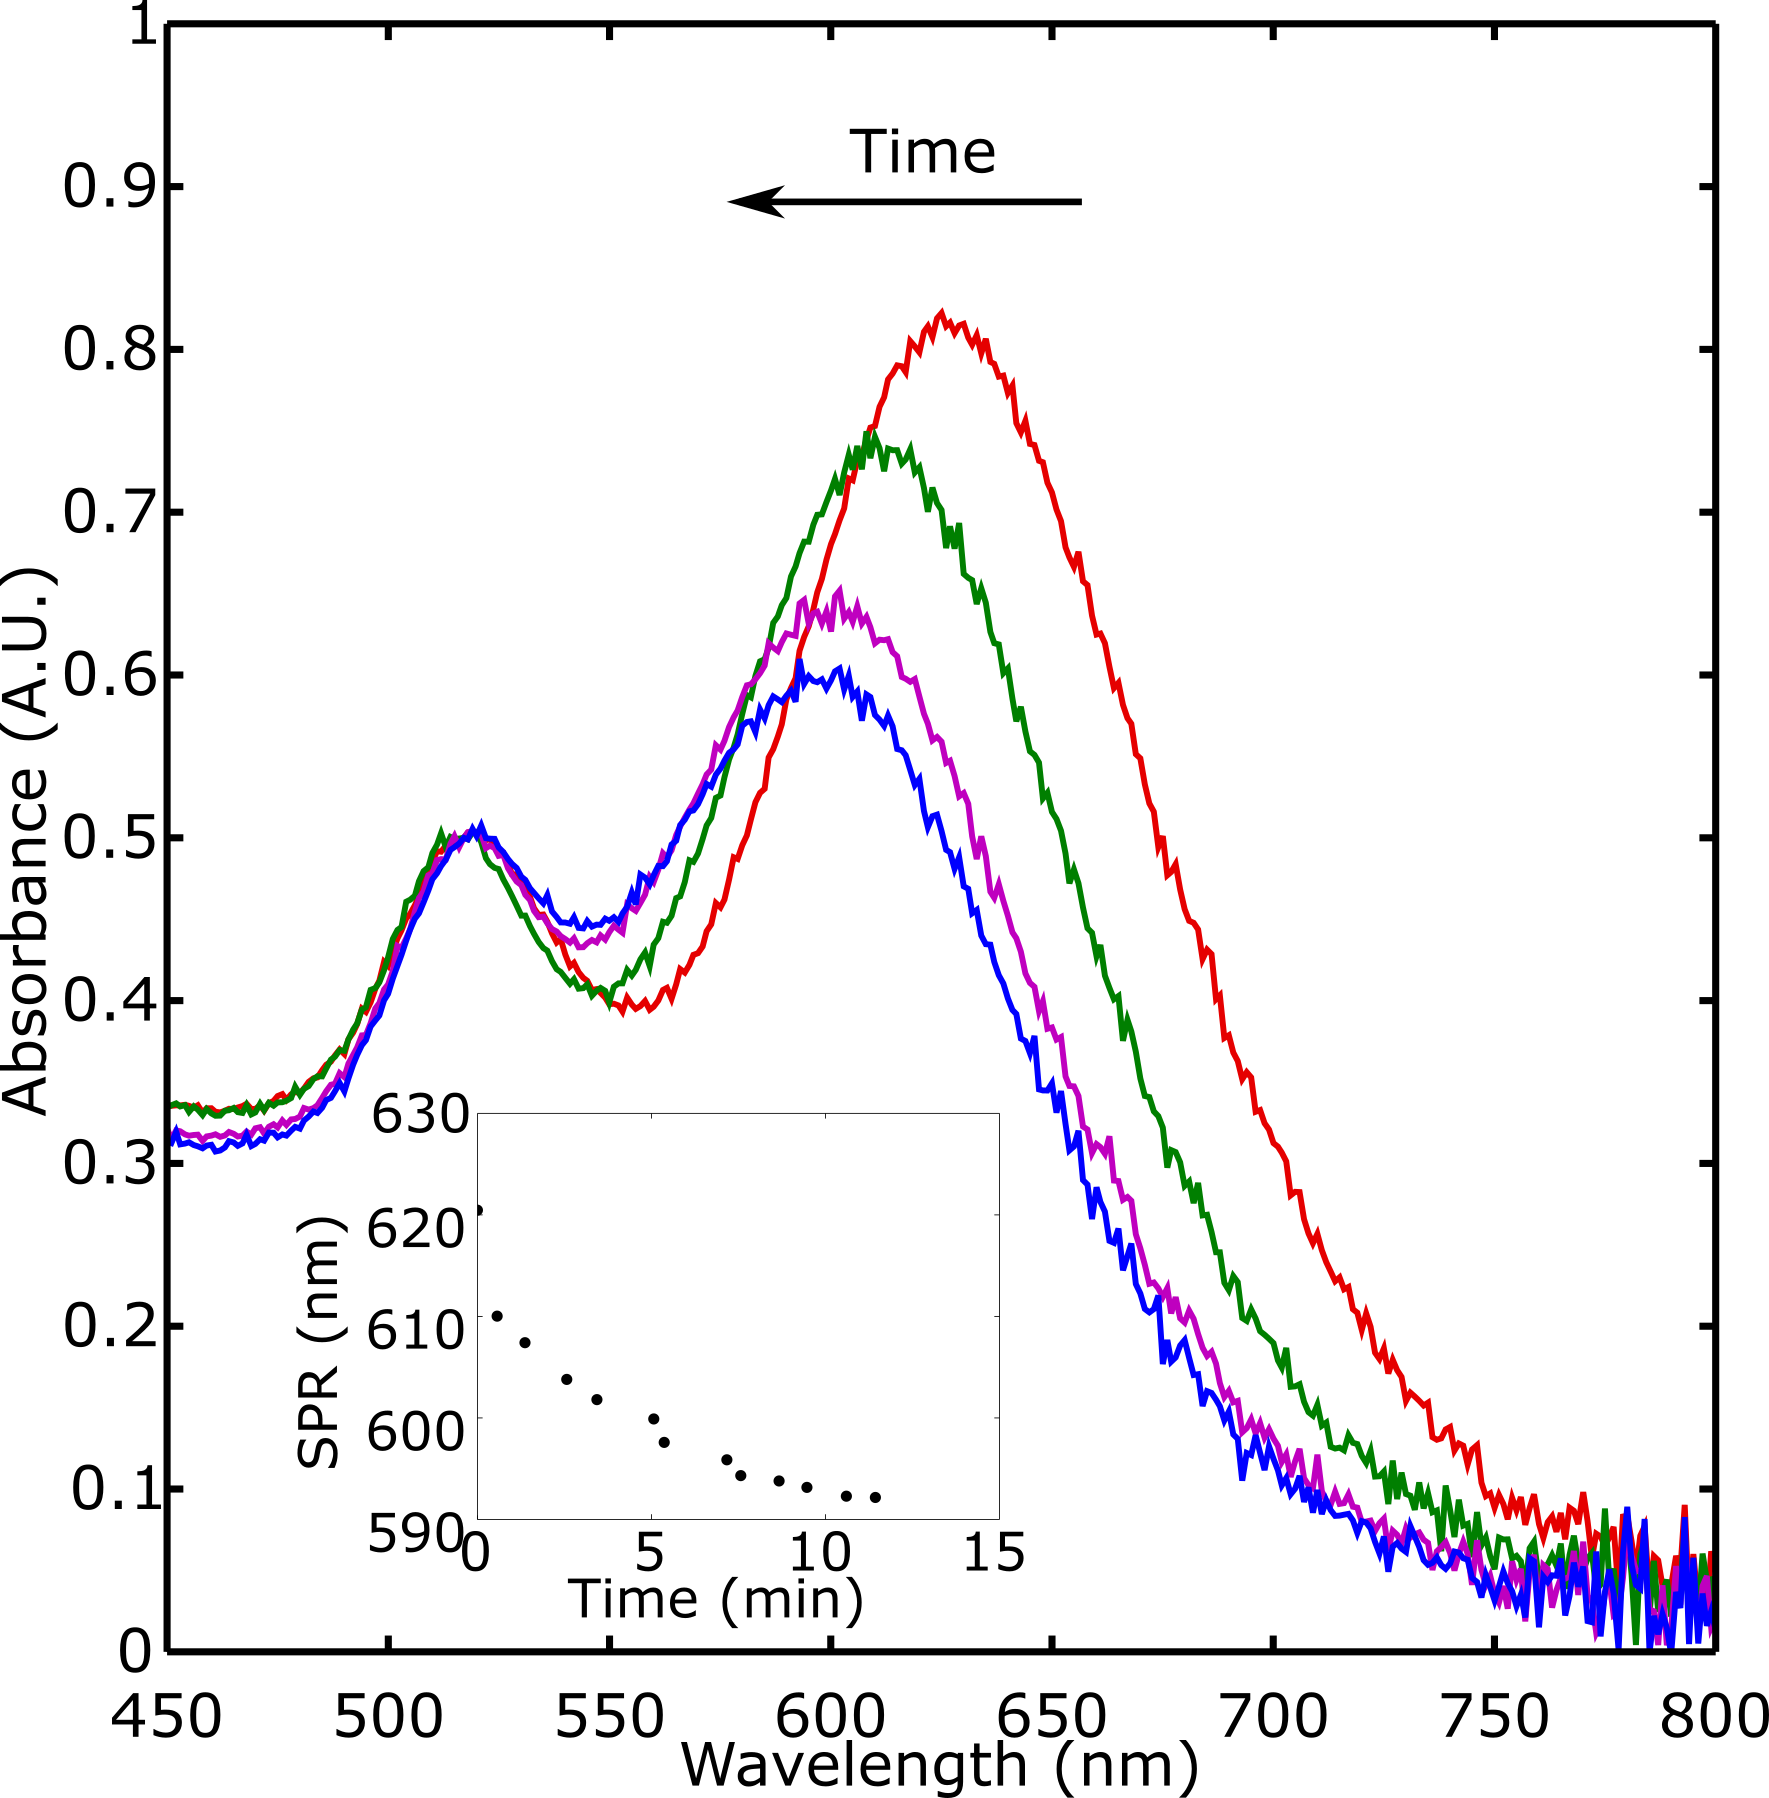
\includegraphics[width=0.45\textwidth]{Chapters/02_KCN/Figures/04_Supporting/01_Bulk/01_bulk.png}
 \caption{Extinction spectra of a bulk suspension of gold nanorods dispersed in
 $100\uM$ KCN. The curves are displayed at 2 minutes intervals. The
 inset shows the peak position as a function of time. The curves were normalized
 to the transverse peak for clarity.}
 \label{fig:Bulk}
\end{figure}

Figure S\ref{fig:Bulk} shows the behavior of nanorods dispersed in $100\uM$ KCN.
The same sample than for the single-particle experiments was used.
We observe a clear blue shift of the longitudinal plasmon resonance, towards the
transverse peak at around $530\nm$. As stated in the main text, we attribute the
blue shift of the peak to a shortening of the long axis of the rods. This is
because the CTAB is more efficient in protecting the sides than the tips of the
particles. The blue shift does not seem stabilized for the last spectrum. We
attribute this to a complete consumption of KCN by excess gold metal in our
sample. If more KCN had been added, the blue-shift would probably have
continued.

The spectra were acquired in an UV-Vis spectrometer. The first spectrum was
acquired with the rods dispersed in water, before adding KCN into the cuvette.
Later a solution such that the final concentration was $100\uM$ was added and a
set of automatic spectra was recorded at a fixed interval of time. The peak
position was extracted by fitting a double Lorentzian, one with a fixed central
wavelength (the transverse resonance) and a second one for the longitudinal
plasmon.


\section{SEM Images}

\begin{figure}[htp]
 \centering
 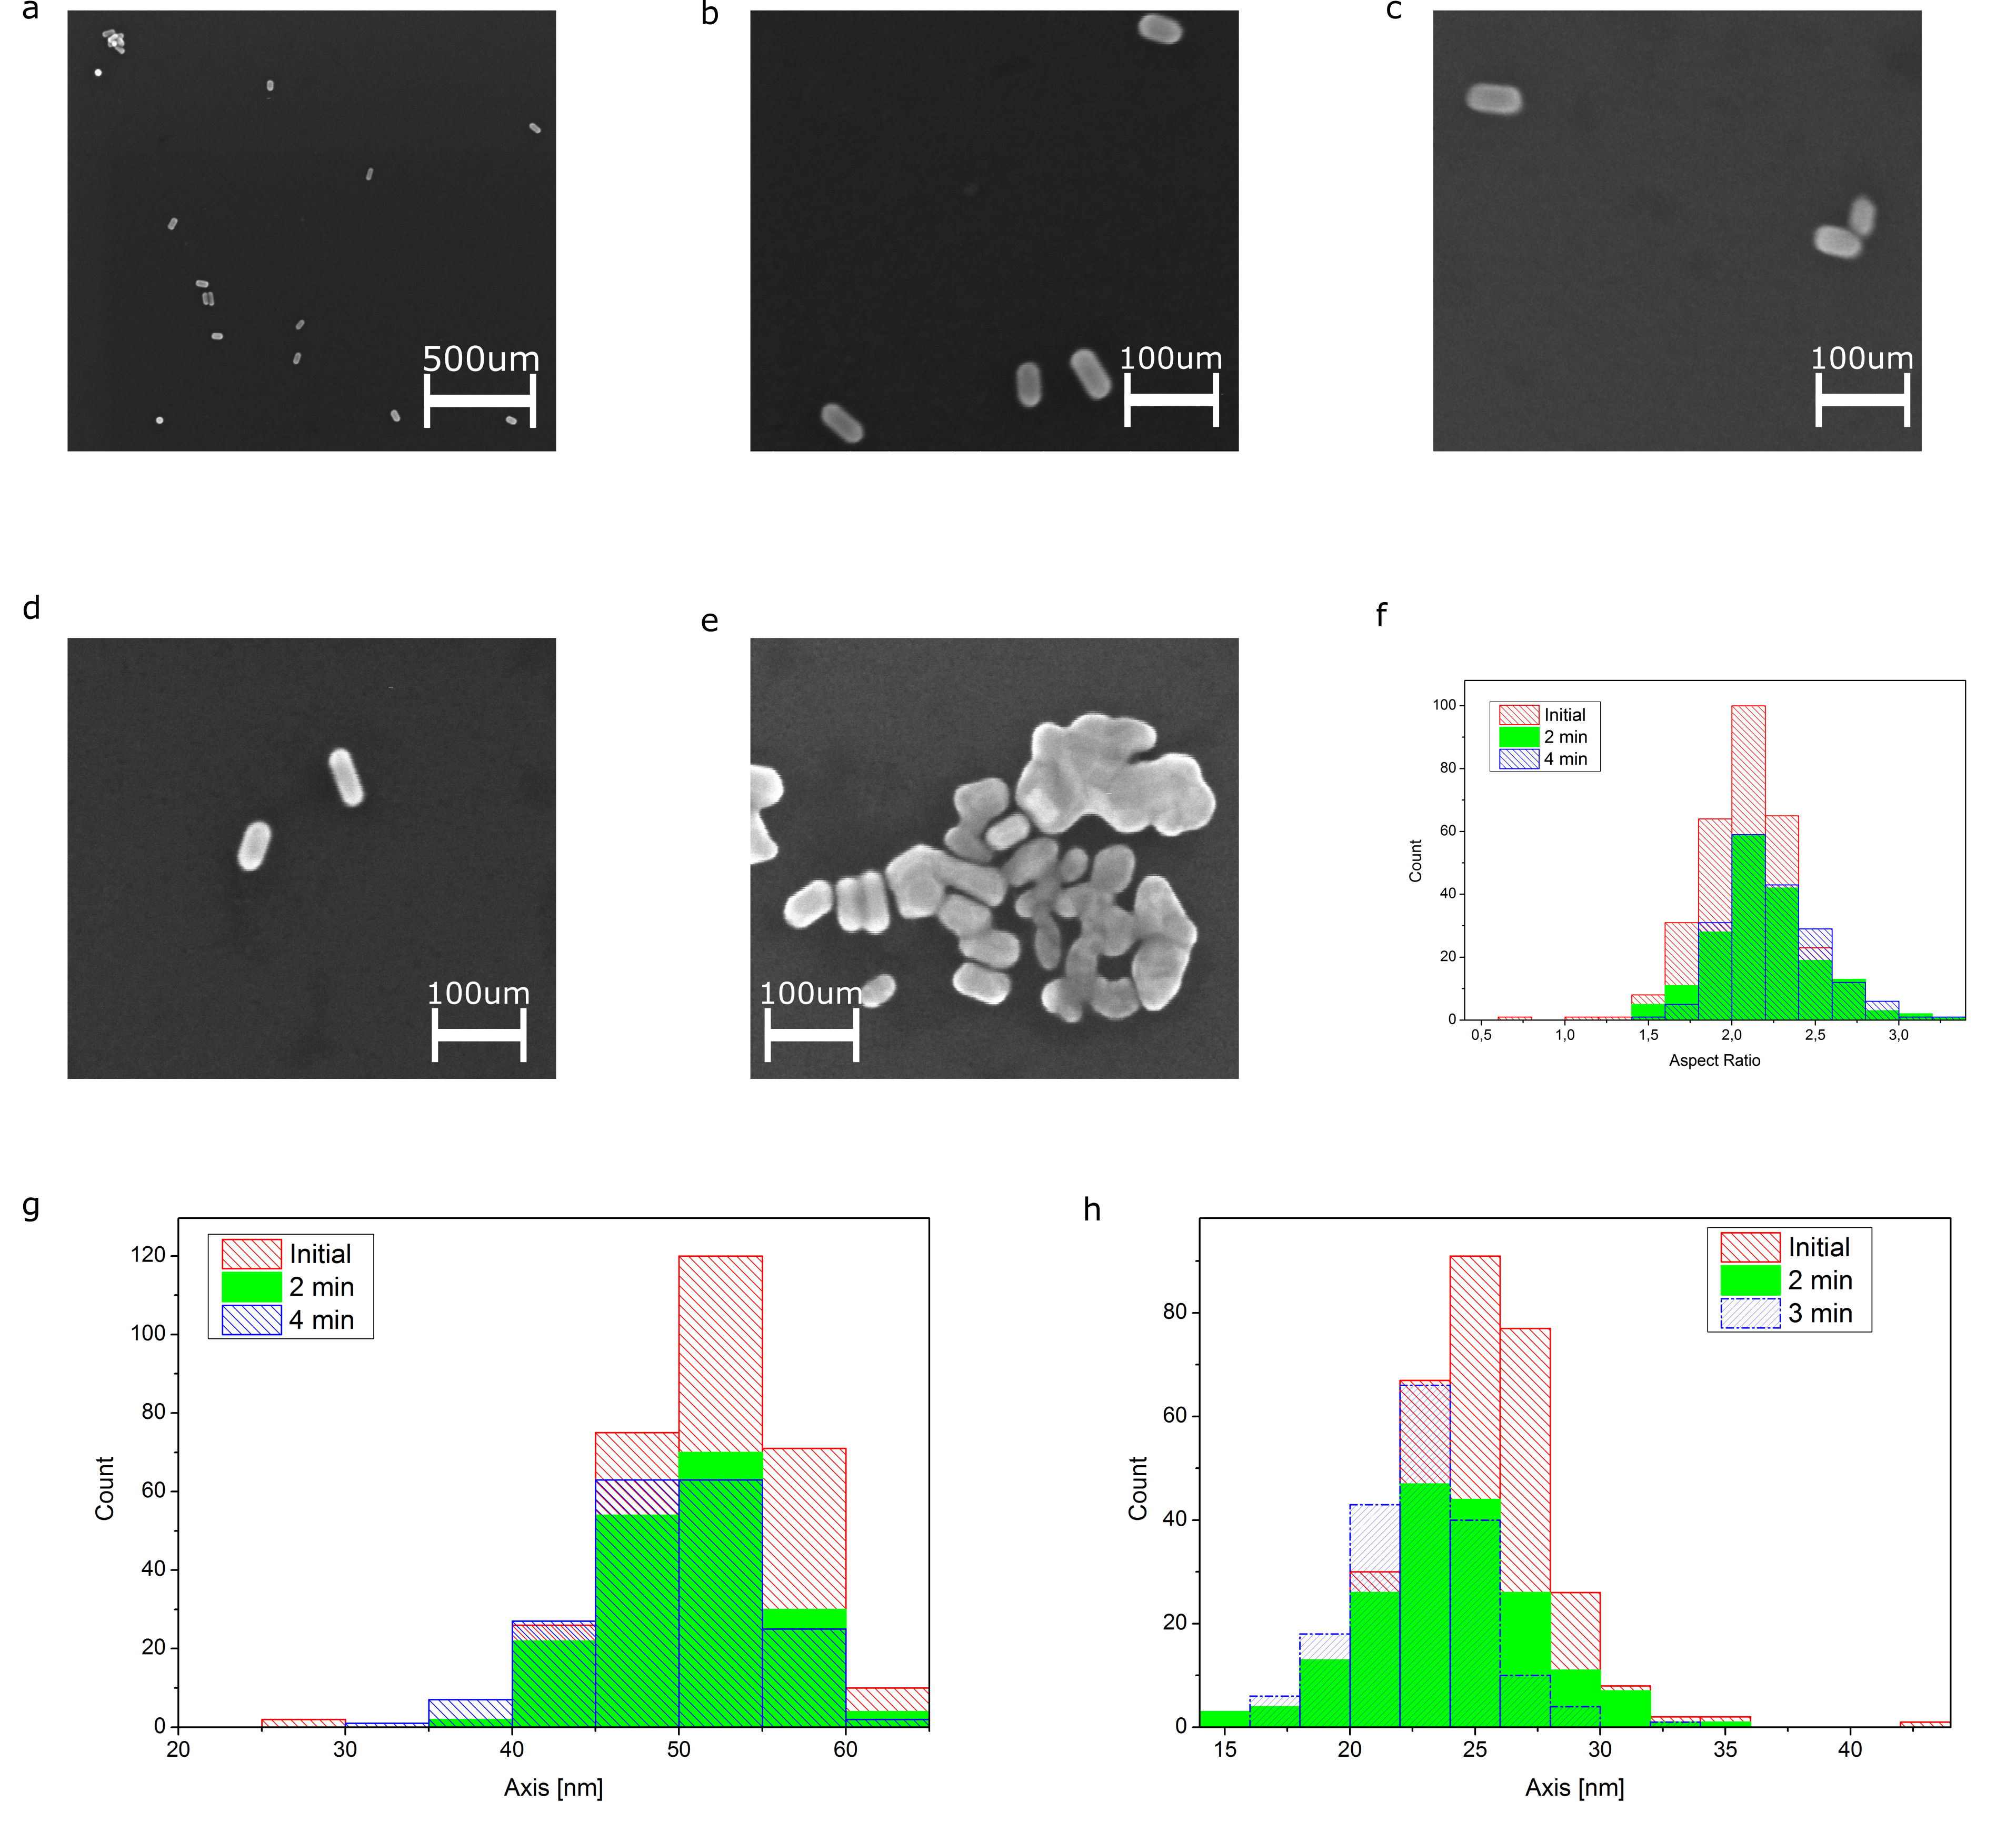
\includegraphics[width=0.95\textwidth]{Chapters/02_KCN/Figures/04_Supporting/02_SEM/sem.png}
 \caption{SEM images of the rods a-b) after synthesis, at different
 magnifications c) after $2$ minutes in $20\uM$ KCN. d) after $4$ minutes in KCN
 and e) when they were forming clusters. f-h) Histograms of the aspect ratio
 (f), longitudinal(g) and transverse axis(h) before, after $2$ and after $4$
 minutes in KCN. The distribution of values is too broad to visualize a shift in
 aspect ratio.
 Statistics on the values, however, show a slight increase and the data is
 summarized in table 1. }
 \label{fig:SEM}
\end{figure}

Samples for SEM images were prepared by drop casting a suspension of gold
nanorods into clean silicon wafers. An initial image of several hundreds of rods
was acquired before any etching. The same samples were placed in a solution of KCN
for $2$ minutes and imaged again. Finally they were submersed again for $2$
minutes in KCN and imaged afterwards. In this way, even if it was not possible
to track the same particles during the etching process, it was possible to
reproduce the conditions in which the reshaping took place on the optical
microscope.

Figure S\ref{fig:SEM} shows the SEM images of the rods. In S\ref{fig:SEM}a,b an
example of the rods after synthesis and before etching at two different
magnificatins. Figures S\ref{fig:SEM}c and d show the rods after $2$ minutes and
$4$ minutes in $20\uM$ KCN. Figure S\ref{fig:SEM}e was acquired after $4$
minutes in KCN; the difference on the shape of the particles when they are in
contact is notable. It has to be reminded however that the clusters of rods were
already formed on the substrate before the etching started. Drop casting a
suspension of rods tends to form conglomerates of particles rather than isolated
particles as can be easily achieved by spin casting and shown in the optical
experiments in the main text.

Histograms in Figures S\ref{fig:SEM}f-h show the
analysis of the aspect ratio, the longitudinal and the transverse axes
respectively for each of the cases. Table 1 summarizes the average values found
after analyzing approximately $300$ particles. The shift is rather small as
compared to the standard deviation of the distribution of sizes. 

\begin{table}[htp]
\begin{tabular*}{0.48\textwidth}{c c c c c}
 $\,$ & L (nm) & Sdv (nm) & D (nm) & Sdv (nm) \\\hline
 $0\textrm{min}$ & $51$ & $5$ & $24$ & $3$ \\
 $2\textrm{min}$ & $50$ & $5$ & $23$ & $3$ \\
 $4\textrm{min}$ & $49$ & $5$ & $22$ & $2$ \\
\end{tabular*}
\label{tab:SEM_results}
\caption{Summary of the results obtained for 300 different particles while
imaging them with an SEM. L and D are the length and diameter respectively.
Sdv is the standard deviation of the values}
\end{table}

\section{Background Spectrum}
\begin{figure}[htp]
 \centering
 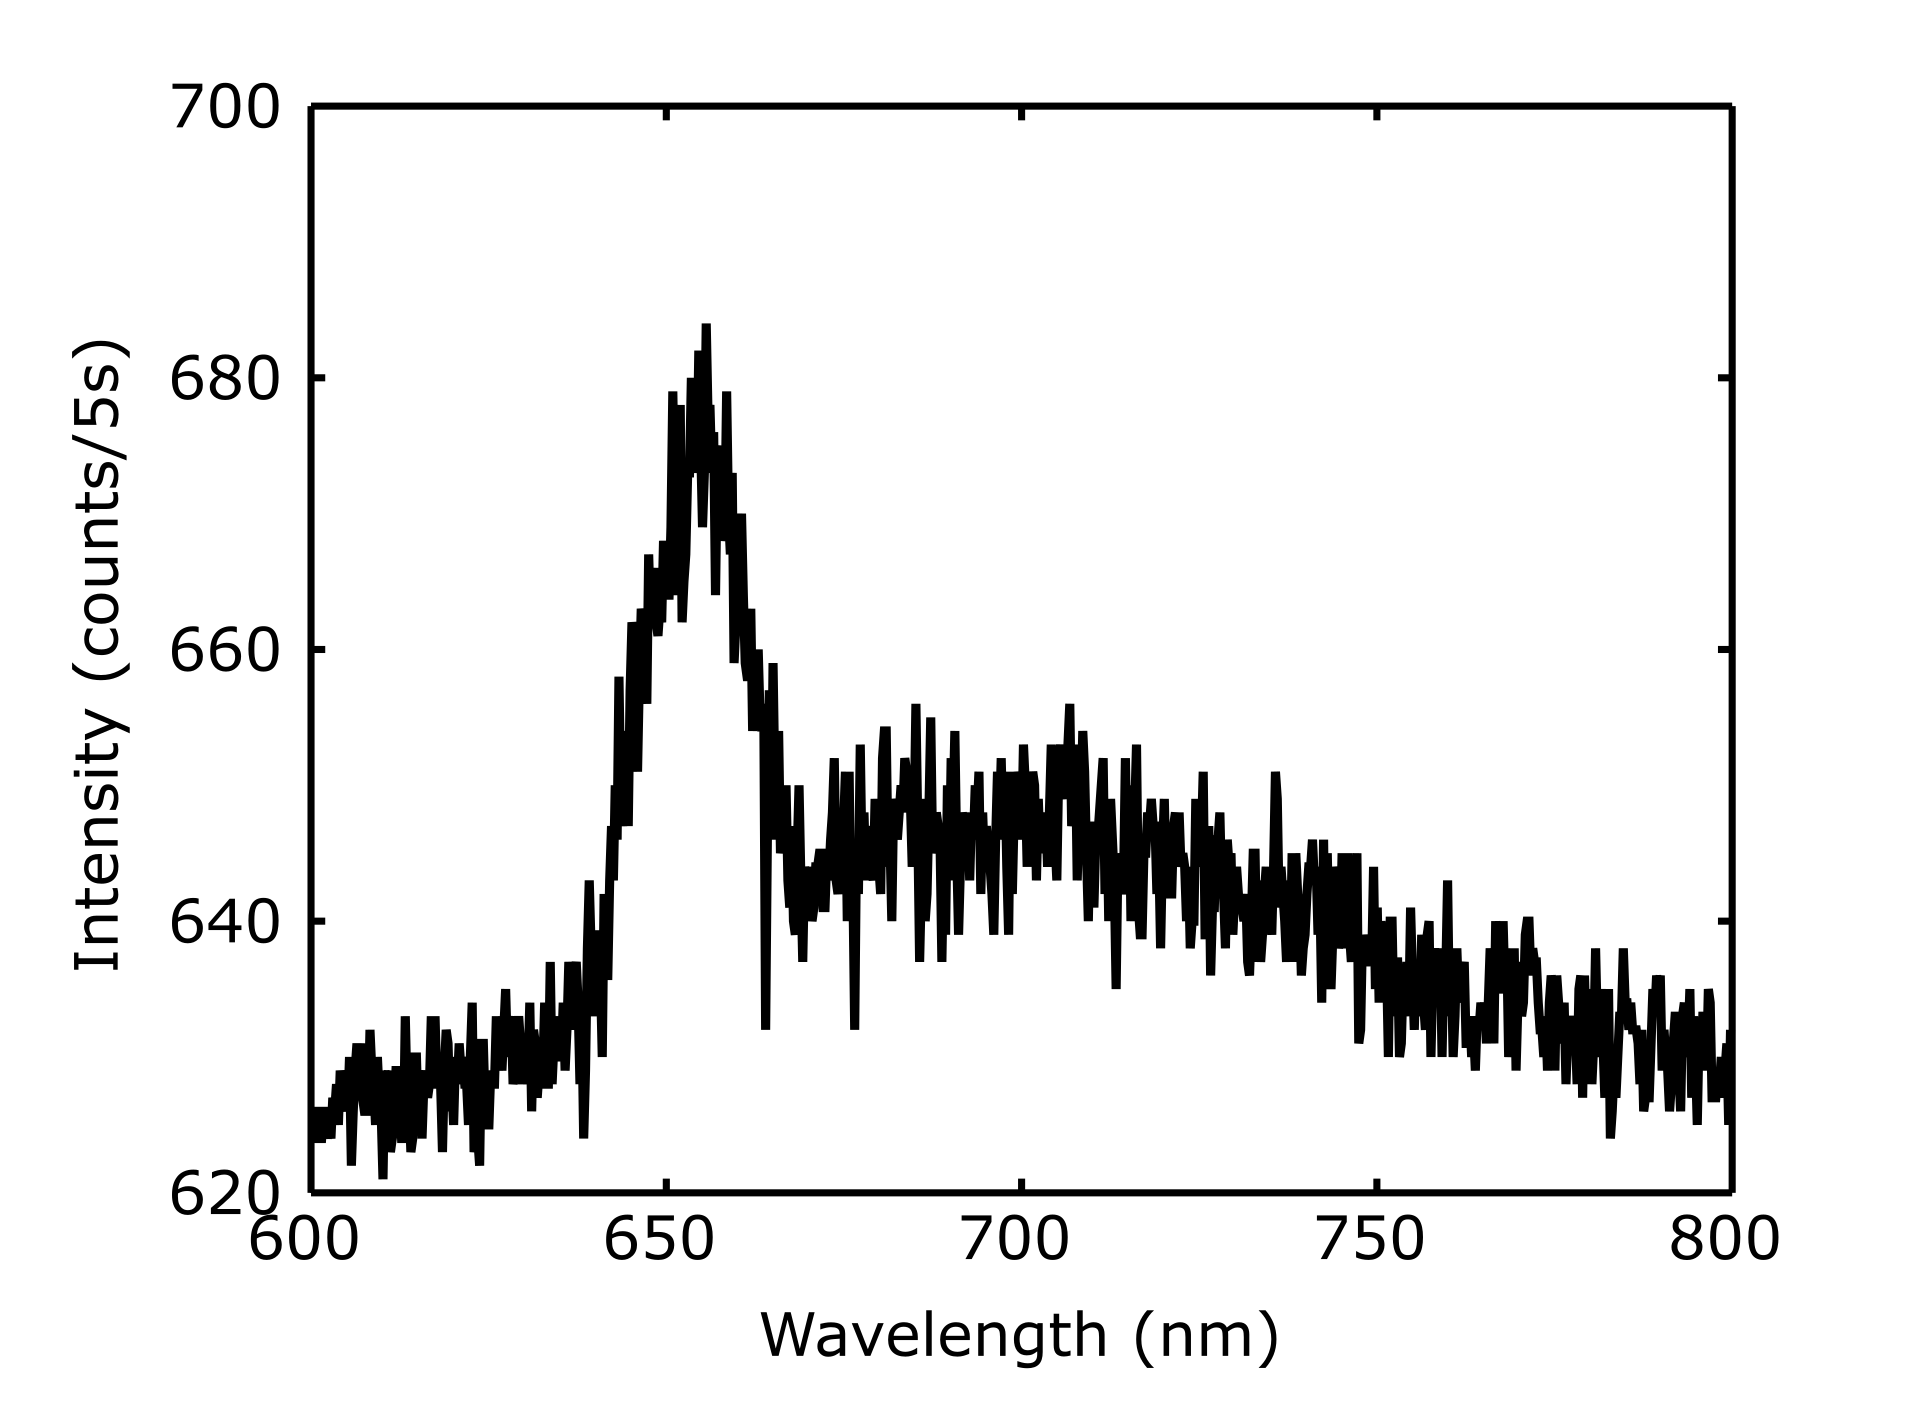
\includegraphics[width=0.95\textwidth]{Chapters/02_KCN/Figures/04_Supporting/03_Background/background.png}
 \caption{Spectra from the background while exciting with a $532\nm$ laser. The
 peak appearing at $650\nm$ is attributed to Raman scattering from the O-H stretching modes of water.}
 \label{fig:Background}
\end{figure}

Figure S\ref{fig:Background} shows the typical background when exciting with a
$532\nm$ laser. The peak at $650\nm$ is attributed to Raman scattering from
water. Normally this background can be well subtracted from the spectra acquired
on particles. For less intense curves however, it is possible to observe a
shoulder appearing at this particular wavelength. This indicates a non-additive
phenomenon that we attributed to enhanced Raman scattering close to the
nanoparticles.